\documentclass[11pt,a4paper,latin1, frenchb]{report}
\usepackage {babel}

% Pour pouvoir utiliser 
%\usepackage{ucs}
\usepackage[T1]{fontenc}
\usepackage[latin1]{inputenc}
\usepackage {lmodern}
\usepackage {picins} %image avec texte a ct
\usepackage{url} % Pour avoir de belles url
\usepackage {geometry}
%\usepackage{slashbox} %backslash dans tableau
%\usepackage[table]{xcolor} %couleur tableau
\usepackage{colortbl,hhline}
\usepackage{color}
\usepackage {listings} % Pour mettre du code source
\usepackage{lscape} %Pour pouvoir passer en paysage
%\usepackage {multicol} %Pour pouvoir faire plusieurs colonnes
%\usepackage{eurosym} %symbole euro
\usepackage{graphicx}
\usepackage{makeidx} %Pour crer un index
%\usepackage {setspace} %Pour l'interligne de 1.5
%\usepackage{shorttoc} %Pour crer un sommaire
\usepackage{caption}
\usepackage[font=scriptsize, format=hang]{subcaption}
\usepackage[babel=true]{csquotes}
\usepackage[toc,page]{appendix}
%\usepackage{subfig}


\setlength{\topmargin}{-6mm}
\setlength{\textheight}{230mm}
\setlength{\textwidth}{160mm}
\setlength{\evensidemargin}{-5.45mm}
\setlength{\oddsidemargin}{-5.45mm}
 
\renewcommand{\no}{n\textsuperscript{o}}
\renewcommand{\nos}{n\textsuperscript{os}}

\renewcommand{\labelitemi}{---}
\renewcommand{\labelitemii}{$\star$}

\renewcommand{\appendixtocname}{Annexes}
\renewcommand{\appendixpagename}{Annexes}

\usepackage[pdftex, 					% Paramtrage de la navigation
bookmarks = true, 						% Signets
bookmarksnumbered = true, 				% Signets numrots
pdfpagemode = UseOutlines, 					% None, UseThumbs, UseOutlines, Fullscreen
pdfstartview = Fit, 					% FitH, FitV, FitR, FitB, FitBH, FitBV, Fit
pdfpagelayout = SinglePage, 				% SinglePage, OneColumn, TwoColumnLeft, TwoColumnRight
colorlinks = false, 					% Liens en couleur
urlcolor = black, 						% Couleur des liens externes
pdfborder = {0 0 0} 					% Style de bordure : ici, rien
]{hyperref}


\hypersetup{
    unicode=false,          % non-Latin characters in Acrobat's bookmarks
    pdftoolbar=true,        % show Acrobat's toolbar?
    pdfmenubar=true,        % show Acrobat's menu?
    pdffitwindow=true,     % window fit to page when opened
    pdftitle={Rapport de projet tuteur�},    % title
    pdfauthor={Pinto Dos Santos Almeida Catherine, Meilhac Beno�t},     % author
    pdfsubject={Transformation d'un diagramme de s�quences SysML vers les automates d'interfaces et v�rification de compatibilit� avec l'outil Ticc},   % subject of the document
    pdfcreator={Pinto Dos Santos Almeida Catherine, Meilhac Benoit},   % creator of the document
    pdfproducer={Texlive (pdflatex)}, % producer of the document
    pdfnewwindow=true,      % links in new window
}


\graphicspath{{images/}}
\newcommand{\sommaire}{\shorttoc{Sommaire}{0}}
\makeindex
\definecolor{grisclair}{gray}{0.75}
\definecolor{orange}{rgb}{1,0.5,0}
\definecolor{vert}{rgb}{0,0.75,0}


% Pour les marges de la page
%\geometry{a4paper, top=2.5cm, bottom=3.5cm, left=1.5cm, right=1.5cm, marginparwidth=1.2cm}
\geometry{a4paper}

% Pour les entetes de page
\usepackage{fancyhdr}


\parskip=5pt %% distance entre les (paragraphe)
\sloppy %% respecter toujours la marge de droite 

% Pour les p�nalit�s :
\interfootnotelinepenalty=150 %note de bas de page
\widowpenalty=150 %% veuves et orphelines
\clubpenalty=150 

%Pour la longueur de l'indentation des paragraphes
\setlength{\parindent}{15mm}

%%%% debut macro pour enlever le nom chapitre %%%%
\makeatletter
\def\@makechapterhead#1{%
  \vspace*{50\p@}%
  {\parindent \z@ \raggedright \normalfont
    \interlinepenalty\@M
    \ifnum \c@secnumdepth >\m@ne
        \Huge\bfseries \thechapter\quad
    \fi
    \Huge \bfseries #1\par\nobreak
    \vskip 40\p@
  }}

\def\@makeschapterhead#1{%
  \vspace*{50\p@}%
  {\parindent \z@ \raggedright
    \normalfont
    \interlinepenalty\@M
    \Huge \bfseries  #1\par\nobreak
    \vskip 40\p@
  }}
\makeatother
%%%% fin macro %%%%

%redfinition maketitle pour mettre en haut de page
\makeatletter
\renewcommand{\maketitle}{%
    \vspace*{0.5cm}% ICI La taille que tu veux avant le titre
    
    \begin{center}%
    {\large
     \lineskip .75em%
      \begin{tabular}[t]{c}%
        \@author
      \end{tabular}\par}%
    \vskip 2em%
    
    {\large \@date \par}%       % Set date in \large size.
    
      \vskip 1.5em%
    {\textbf{\LARGE \@title} \par}%
    \end{center}\par
    \vskip 1.5em%
	\thispagestyle{empty}% virer numrotation
	\setcounter{page}{0}% remettre compteur au dbut
	\clearpage
	\newpage
}
\makeatother

%Couverture 

\title{
	\normalsize{D�partement informatique\\
	Universit� de Franche-Comt�\\
	Projet tuteur�\\
	Ann�e 2011-2012}\\
	\vspace{15mm}
}

\author{
    Catherine PINTO DOS SANTOS ALMEIDA\\Beno�t MEILHAC  %rajouter un \\ au besoin
	\vspace{5mm}
}

\date{
	\begin{center} 
        
\includegraphics[scale=0.15]{ufc.jpg}
	\end{center}
	\vspace{5mm}
	\huge{\textbf{Transformation de diagrammes de s�quences SysML vers les automates d'interfaces et v�rification de la compatibilit� avec l'outil Ticc}}\\
	\vspace{14mm}
	\normalsize{	
	Tuteurs :\\
        Mr MOUNTASSIR\\
        Mr HAMMAD\\
        Mr CHOUALI
	}
}


\begin{document}
%\maketitle
\begin{titlepage}
    \centering

    \vspace{5mm}

    \begin{center} 
        
\includegraphics[scale=0.20]{ufc.jpg}
	\end{center}
	
    \vspace{5mm}
	
    \Huge{
        \textbf{
            Transformation de diagrammes de s�quences SysML vers les automates d'interfaces et v�rification de la compatibilit� avec l'outil Ticc
        }
    }
	
    \vspace{14mm}
 
    \normalsize{
        Catherine PINTO DOS SANTOS ALMEIDA\\Beno�t MEILHAC
    }

	\vspace{5mm}

	\normalsize{	
	    Tuteurs :\\
        Mr MOUNTASSIR\\
        Mr HAMMAD\\
        Mr CHOUALI
	}

	\vspace{20mm}

    \normalsize{
        \textbf{
            D�partement informatique\\
        	Universit� de Franche-Comt�\\
            Projet tuteur�\\
        	Ann�e 2011-2012
        }
    }

\end{titlepage}

\clearpage


\chapter*{Remerciements}
\phantomsection

En premier lieu, nous tenons {\`a} remercier nos tuteurs, Monsieur Mountassir, Monsieur Hammad, ainsi que Monsieur Chouali pour leur aide, leur soutien et leur efficacit{\'e} tout au long du projet.\\

Nous adressons ensuite nos remerciements {\`a} l'{\'e}quipe enseignante gr{\^a}ce {\`a} qui nous avons p{\^u} acqu{\'e}rir les comp{\'e}tences n{\'e}cessaires {\`a} la r{\'e}alisation du projet.\\

Finalement, nous remercions nos relecteurs pour leur patience et leur gentillesse.


\clearpage

\addtocontents{toc}{\protect\thispagestyle{empty}}
\tableofcontents

\clearpage

\setcounter{page}{1} 

\pagestyle{fancy}
\renewcommand{\chaptermark}[1]{\markboth{#1}{}} 
\renewcommand{\sectionmark}[1]{\markright{#1}} 

\chapter{Introduction}

De mani�re g�n�rale, pour fiabiliser le fonctionnement d'un syst�me avant son implantation sur une machine, on doit l'�tudier en amont. 

Les  phases de sp�cification et de v�rification sont devenues incontournables dans le cycle de vie pour du logiciel dans l'industrie. 

C'est pour ces raisons que l'on doit parler de la v�rification de sys�mes pour augmenter le degr� de confiance dans leur fonctionnement futur. 

En ce qui concerne le projet, il est int�ressant de s'int�resser � des syt�mes bas�s sur une architecture � composants. Avant le d�ploiment sur une machine, il est important de v�rifier dans un premier temps sa coh�rence et en particulier la compatibilit� entre composants.

SysML\protect\footnote{System Modeling Language} est une extension du langage UML\protect\footnote{Unified Modeling Language} sp�cialis� dans la mod�lisation, la sp�cification et la documentation de syst�mes. 
Les am�liorations qu'il apporte par rapport � UML lui ont permis d'accro�tre sa popularit� tant dans l'industrie que dans le milieu universitaire.
SysML introduit de nouveaux concepts comme la disparition des classes UML au profit de blocs qui sont l'unit� de base de la structure d'un syst�me (logiciel ou mat�riel). Ainsi le diagramme de classes UML est remplac� par le diagramme de d�finition de blocs (BDD\protect\footnote{Block Definition Diagram}). Celui-ci met en avant la hi�rarchie du syst�me et les diff�rentes interactions entre les composants.
Ces interactions peuvent �tre repr�sent�es sous forme d'un diagramme de s�quences mod�lisant les �changes de messages dans le temps.
Cependant, la mod�lisation ne permet pas � elle seule de v�rifier et valider la compatibilit� des composants entre eux.

Dans un mod�le bas� sur les composants, la v�rification de compatibilit� entre composants est introduite par la notion d'automates d'interfaces. Ils servent � d�crire les diff�rentes interactions d'entr�es/sorties donc le comportement d'un composant avec son environnement.

C'est dans ce contexte que se situe le projet. Partant d'un diagramme de d�finition de blocs, tous les blocs ayant des interactions avec d'autres donnent acc�s � des diagrammes de s�quences associ�s. Ces diagrammes sont ensuite transform�s en automates d'interfaces. Une v�rification de leur compatibilit� est alors possible.

Dans un premier temps, une premi�re partie sera consacr�e � fixer le cadre du projet ainsi que les diff�rents outils qui ont �t� utilis�s. Ensuite, une deuxi�me partie exposera la mise en \oe{}uvre du projet. Et en dernier lieu, les diff�rents probl�mes qui ont �t� rencontr�s.

\clearpage



\definecolor{gris}{gray}{0.5}
\lstset{
	numbers=left,
	numberstyle=\footnotesize,
%	numberstyle=Sepia,
	stepnumber=2,
	numbersep=5pt,
	frame=shadowbox,
	backgroundcolor=\color{grisclair},
	rulesepcolor=\color{gris}
}

\chapter{Pr�liminaires}

\section{SysML : System Modeling Language}

\subsection{Contexte}

Les m�thodes de l'Ing�nierie Syst�me (IS) reposent sur des approches de mod�lisation et de simulation pour valider les exigences, et pour v�rifier ou �valuer le syst�me. La mod�lisation a donc couramment �t� utilis�e pour l'IS, que ce soit pour des repr�sentations concr�tes avec des plans ou mod�les r�duits, ou plus abstraites avec des syst�mes d'�quations.\\
Les sp�cifications issues de l'IS produisant souvent une documentation tr�s dense, une fa�on de la simplifier est d'utiliser une approche orient{\'e}e mod�les. Elle permet de r{\'e}aliser un mod{\`e}le coh�rent du syst{\`e}me, stock{\'e} et g{\'e}r{\'e} dans un r{\'e}f{\'e}rentiel.\\
La mod{\'e}lisation permet de ma{\^i}triser la complexit{\'e} du syst{\`e}me {\'e}tudi{\'e}, car chaque mod{\`e}le donne acc{\`e}s {\`a} une repr{\'e}sentation abstraite de diff{\'e}rents aspects du syst{\`e}me.

\subsection{Pourquoi SysML ?}

La mod{\'e}lisation avec le langage UML~\cite{siteUML} est une pratique bien {\'e}tablie dans l'industrie logicielle. Bien que le langage UML permet par son caract{\`e}re {\`a} usage g{\'e}n{\'e}ral d'adresser de nombreux besoins pour l'IS, il ne r{\'e}pond pas {\`a} tous les besoins.\\
SysML apporte une simplification et une standardisation du vocabulaire, plus question ici de classes, d'objets, ou d'h{\'e}ritages. Ce nouveau langage, ajoute aussi la possibilit{\'e} de repr{\'e}senter les exigences du syst{\`e}me comme elles sont d{\'e}finies dans un cahier des charges, les {\'e}l{\'e}ments non-logiciels (m{\'e}canique, hydraulique, capteur \dots), les {\'e}quations physiques, les flux continus (mati{\`e}re, {\'e}nergie, etc.) et les allocations.

\subsection{SysML}

Systems Modeling Language (SysML~\cite{siteSysML}) est bas{\'e} sur UML et remplace la mod{\'e}lisation de classes et d'objets par la mod{\'e}lisation de blocs pour un vocabulaire plus adapt{\'e} {\`a} l'Ing{\'e}nierie Syst{\`e}me. Un bloc englobe tout concept logiciel, mat{\'e}riel, donn{\'e}es, processus, et m{\^e}me la gestion des personnes.

Le projet SysML a {\'e}t{\'e} men{\'e} conjointement entre l'INCOSE~\cite{siteINCOSE} (International Council on Systems Engineering) et l'OMG (Object Management Group), organisme responsable d'UML, et a {\'e}t{\'e} valid{\'e} en 2006. Depuis il fut repris jusque arriver {\`a} une \textit{Final Adopted Specification} telle que le d{\'e}fini l'OMG~\cite{siteOMG}. La version actuelle (1.2) date de juin 2010.

\subsection{Diff{\'e}rences entre SysML et UML}

SysML r{\'e}utilise certaines fonctionnalit{\'e}s d'UML mais en les simplifiant en plus d'en int{\'e}grer de nouvelles. 
\noindent Ce qui peut {\^e}tre repr{\'e}sent{\'e} sous la forme du diagramme pr�sent� par la figure~\ref{UMLSysML} ci-dessous.

\begin{figure}[!ht]
	\centering
	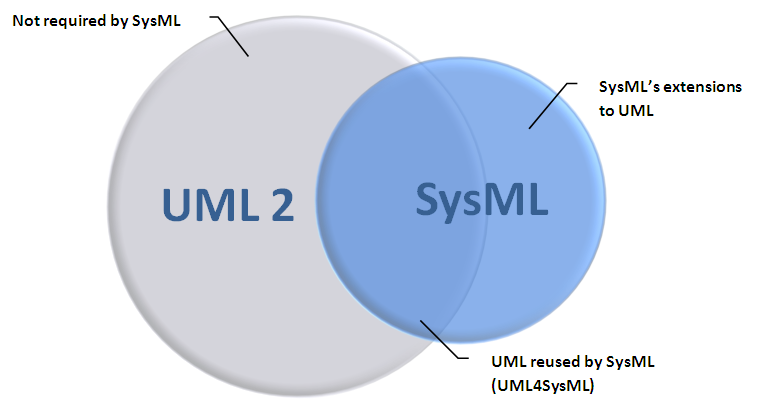
\includegraphics[scale=0.6]{image3.png}
	\caption{UML vs SysML}
	\label{UMLSysML}

\end{figure}

\noindent UML4SysML :
\begin{itemize}
	\item diagramme de s{\'e}quences;
	\item diagramme d'{\'e}tats;
	\item diagramme de cas d'utilisations;
	\item diagramme d'activit{\'e}s;
	\item diagramme de paquetage;
	\item diagrammes de classe et structure composite (utilis{\'e}s pour les diagrammes de d{\'e}finitions de blocs et de bloc interne) BDD\protect\footnote{Block Definition Diagram} \& IDB\protect\footnote{Block Definition Diagram}.

\end{itemize}

\noindent Extensions SysML  :
\begin{itemize}
	\item d{\'e}finitions pour les diagrammes de d{\'e}finitions de blocs et de bloc interne - BDD \& IDB;
	\item modifications dans le diagramme d'activit{\'e}s;
	\item diagramme d'exigences (requirements) - Nouveau;
	\item diagramme param{\'e}trique - Nouveau;
	\item allocations (tra\c{c}abilit{\'e}) - Nouveau.

\end{itemize}


\subsection{Structure de SysML}

SysML comprend donc 9 diagrammes dont 4 sont structurels, 4 dynamiques, et un diagramme d'exigences:
\begin{itemize}
	\item Structurels
	\begin{itemize}
		\renewcommand{\labelitemii}{$\bullet$}
		\item Le BDD remplace le diagramme de classes;
		\item L'IBD remplace le diagramme de structure composite;
		\item Le diagramme de paquetage reste inchang{\'e};
		\item Le diagramme param{\'e}trique est une extension SysML pour l'analyse de param{\`e}tres critiques du syst{\`e}me.

	\end{itemize}
	
	\item Dynamiques
	\begin{itemize}
		\renewcommand{\labelitemii}{$\bullet$}
		\item Le diagramme d'activit{\'e}s est l{\'e}g{\`e}rement modifi{\'e} pour SysML;
		\item Les diagrammes de s{\'e}quences, d'{\'e}tats, et de cas d'utilisations restent inchang{\'e}s.

	\end{itemize}
	
\item Le diagramme d'exigences est une extension SysML.

\end{itemize}

La structure de SysML peut {\^e}tre d{\'e}compos{\'e}e via le diagramme pr�sent� par la figure~\ref{Description des diagrammes SysML}.

\begin{figure}[!ht]
	\centering 
	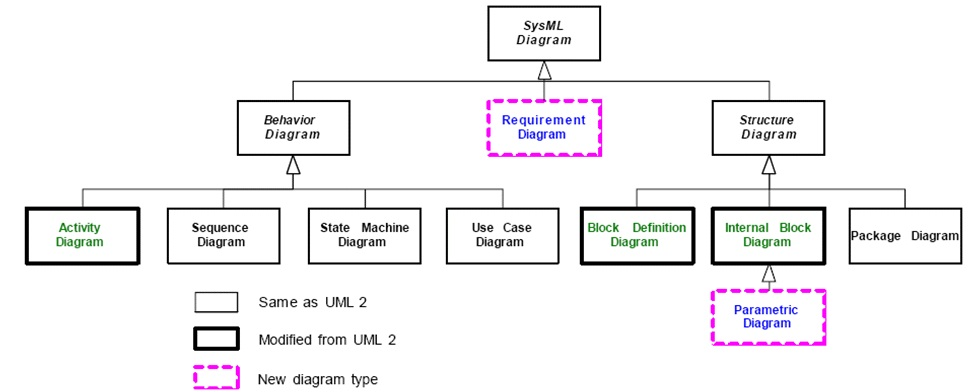
\includegraphics[scale=0.6]{image5.jpg}
	\caption{Description des diagrammes SysML}
	\label{Description des diagrammes SysML}

\end{figure}

\subsection{Exemples de diagrammes}

Afin d'illustrer SysML de fa�on concr{\`e}te, la suite pr{\'e}sentera deux diagrammes repr{\'e}sentatifs : un diagramme BDD et un diagramme IBD.

\subsubsection{Diagramme BDD}
	
Le diagramme BDD repr{\'e}sente une vue d{\^i}te bo{\^i}te noire d'un bloc. Il pr{\'e}sente les blocs et les relations entre eux. Par rapport {\`a} UML, le diagramme BDD red{\'e}fini le diagramme de classes en rempla\c{c}ant les classes par des blocs. 
	
\noindent Le diagramme BDD de la figure~\ref{Exemple de diagramme BDD d'un purificateur d'eau} ci-dessous provient de l'exemple OMG d'un purificateur d'eau.\\

\begin{figure}[!ht]
	\centering 
	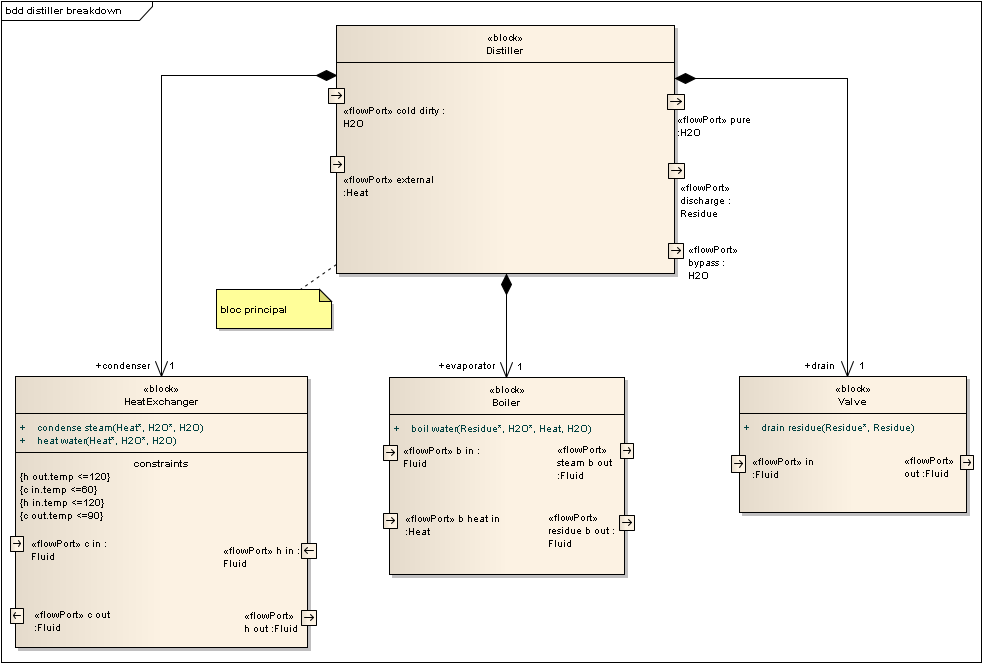
\includegraphics[scale=0.45]{image6.png}
	\caption{Exemple de diagramme BDD d'un purificateur d'eau}
	\label{Exemple de diagramme BDD d'un purificateur d'eau}

\end{figure}

\noindent Les blocs peuvent {\^e}tre en relation les uns avec les autres.\\
Ils ont aussi des ports d'entr{\'e}e/sortie qui permettent de simuler des {\'e}l{\'e}ments requis et fournis entre les blocs. Ainsi, le bloc \enquote{Distiller} a besoin d'eau froide en entr{\'e}e et de chaleur externe pour produire en sortie de l'eau purifi{\'e}e, du r{\'e}sidu, et de l'eau pour le bypass.

\subsubsection{Diagramme IBD} 

Le diagramme IBD repr{\'e}sente la vue bo{\^i}te blanche d'un bloc, c'est-{\`a}-dire la description de la vue interne d'un bloc. Il pr{\'e}sente les blocs composants le bloc principal et la fa\c{c}on dont ils sont assembl{\'e}s ensemble via des ports.  Par rapport {\`a} UML, le diagramme IBD red{\'e}fini le diagramme de structure composite. Le diagramme IBD ci-dessous provient de l'exemple OMG du purificateur d'eau, et correspond au diagramme de d{\'e}finition de bloc BDD pr�sent� par la figure~\ref{Exemple de diagramme BDD d'un purificateur d'eau}.

Le diagramme IBD permet d'obtenir le fonctionnement interne du composant et les interactions des composants qui le composent avec les ports d'entr{\'e}e/sortie. La figure~\ref{Exemple de diagramme IBD du bloc Distiller} pr�sente un exemple de diagramme IBD.

\begin{figure}[!ht]
	\centering 
	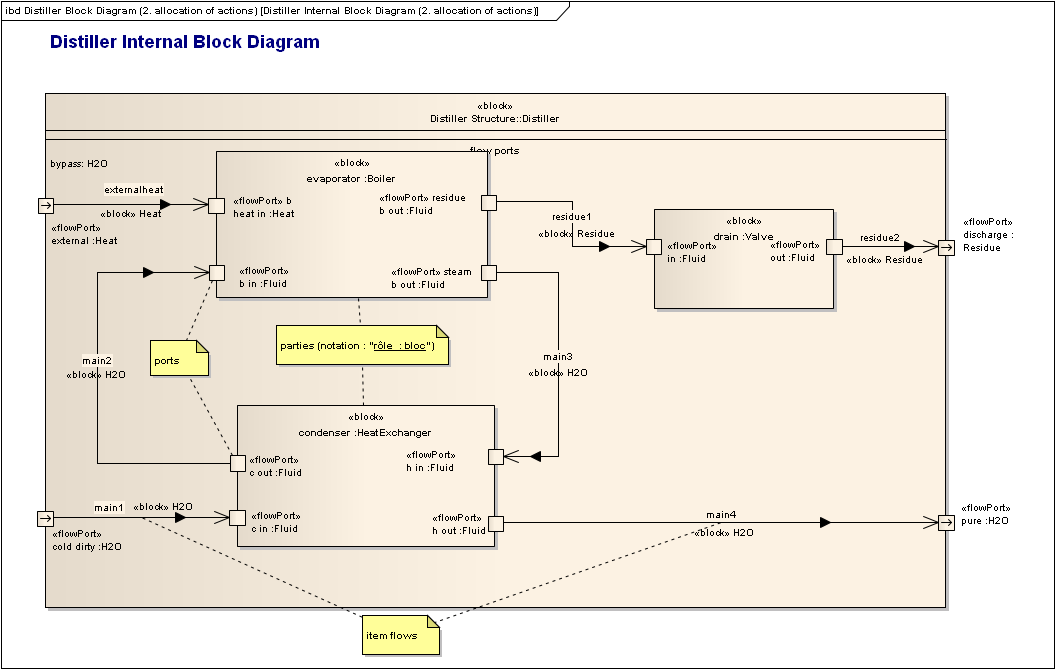
\includegraphics[scale=0.4]{image8.png}
	\caption{Exemple de diagramme IBD du bloc Distiller}
	\label{Exemple de diagramme IBD du bloc Distiller}

\end{figure}

\subsection{Outils SysML}

Le langage SysML a {\'e}t{\'e} int{\'e}gr{\'e} dans de nombreux outils AGL\protect\footnote{Atelier de G�nie Logiciel}, commerciaux ou open source:
\begin{itemize}
	\item Sparx Systems Enterprise Architect (plugin SysML ou version Ultimate requise);
	\item IBM Rational Software Modeler (plugin d'une soci{\'e}t{\'e} tierce disponible);
	\item Magicdraw (plugin SysML requis);
	\item Open source: Topcased (environnement Eclipse).

\end{itemize}

\section{TopCased}

L'IDE\protect\footnote{Integrated Development Environment} Topcased\protect\footnote{Toolkit in Open Source for Critical Applications \& Systems Development}~\cite{siteTopcased} propose des outils int�ressants et facilement exploitables pour l'ing�nierie syst�me. Sont impl�ment�s (ou en cours d'impl�mentation) des moyens d'analyse d'exigences, mod�lisation, simulation de mod�les, impl�mentation, test, validation, r�tro-ing�nierie, g�n�ration de code, de mod�les et de documentation, et gestion de projet.

On le trouve soit sous forme de plugin d'eclipse, soit en tant qu'application RCP\protect\footnote{Rich Client Platform}. Il contient donc un IDE bas� sur le framework de la plate forme de d�veloppement Eclipse, � laquelle il ajoute des fonctionnalit�s essentiellement li�es � la mise en \oe{}uvre de la premi�re branche du cycle en V pour l'ing�nierie du logiciel, du mat�riel ou de syst�mes mixtes logiciel/mat�riel.

S'appuyant principalement sur des langages standardis�s pour la mod�lisation du logiciel (UML, SysML, AADL, \dots{}), Topcased travaille avec des fichiers XMI\protect\footnote{XML Metadata Interchange}. Tous ses standards sont impl�ment�s dans leurs derni�res versions stables, soit directement par le projet Topcased, soit par les modules de la derni�re version stable de la plate-forme Eclipse. Sa derni�re version �tant la 5.1.0, bas�e sur Eclipse 3.7.1 (Indigo). La figure~\ref{exempleModelisationTopcased} montre diff�rentes mod�lisations possibles avec Topcased.

%\clearpage

\begin{figure}[!ht]
	\centering 
	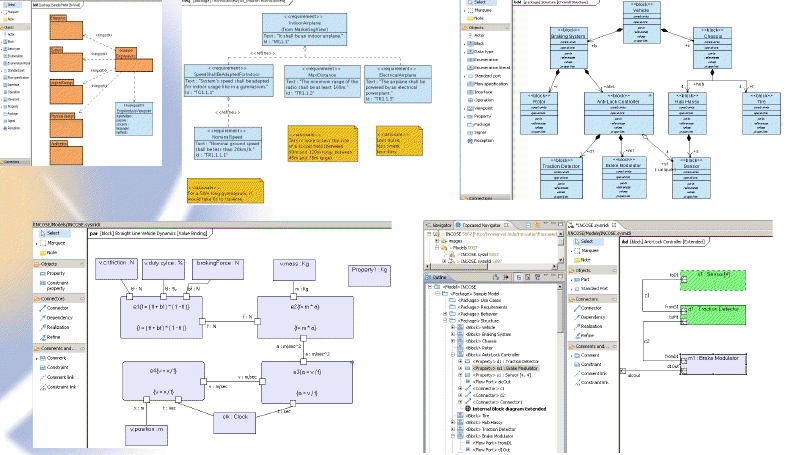
\includegraphics[scale=0.5]{viewer.png}
	\caption{Exemples de mod�lisation avec Topcased}
	\label{exempleModelisationTopcased}

\end{figure}

\section{Ticc}

\subsection{Qu'est ce que Ticc ?}

Ticc~\protect\footnote{Tool for Interface Compatibility and Composition}~\cite{siteTicc, ticcDocumentation} est un outil qui permet de d�finir des interfaces (appel�es modules) et de les composer ensembles. Il est �crit en OCaml et est disponible gratuitement. Il utilise le mod�le � composants d'Alfaro et Henzinger d�fini dans~\ref{sectionAutomateInterface}.

\noindent Ticc fournit les fonctions suivantes :
\begin{itemize}
	\item La mod�lisation des composants de conception et leurs interactions : 
	\begin{itemize}
		\renewcommand{\labelitemii}{$\bullet$}
		\item Chaque composant peut sp�cifier son comportement, ainsi que le comportement attendu des autres composants;
		\item Les fonctionnalit�s du mod�le int�grent des �tats partag�s (via la visibilit� des variables : partag� ou priv�), une communication et une synchronisation uni ou bi-directionnelle (via la synchronisation des actions);
		\item Avantage : il est concis.

	\end{itemize}
	
	\item La composition et la v�rification de la compatibilit� : 
	\begin{itemize}
		\renewcommand{\labelitemii}{$\bullet$}
		\item Lorsque les composants sont assembl�s, Ticc v�rifie qu'ils interagissent correctement;
		\item Ticc est capable de propager les contraintes d'entr�e des composants lors de la composition;
		\item Avantage : la coh�rence du mod�le est assur�e.

	\end{itemize}
	
	\item La simulation et la v�rification :
	\begin{itemize}
		\renewcommand{\labelitemii}{$\bullet$}
		\item Ticc peut v�rifier les propri�t�s CTL\protect\footnote{Computational Tree Logic} des mod�les, ainsi que les simuler;
		\item Ticc s'appuie sur les m�thodes symboliques pour une analyse efficace des espaces d'�tats;
		\item Avantage : la justesse des mod�les et le respect des sp�cifications peuvent �tre v�rifi�es. 

	\end{itemize}  

\end{itemize} 

Cet outil a �t� cr�� par Luca de Alfaro, Bo Adler, Marco Faella, Axel Legay, Vishwanath Raman, Leandro Dias Da Silva, et Pritam Roy. Ticc est en d�veloppement constant, et des versions sont r�guli�rement mises � jour avec de nouvelles fonctionnalit�s. La version actuelle est la 0.3.

\subsection{Un exemple d'utilisation de Ticc}
\label{utilisationTicc}

Afin de pouvoir faire des op�ration sur des mod�les, Ticc doit prendre en entr�e deux fichiers diff�rents : 
\begin{itemize}
	\item un \enquote{.si} : qui contient le mod�le (connut �galement sous \enquote{sociable interface});
	\item un \enquote{.in} : qui contient  le code OCaml qui permet de charger le mod�le et y faire des op�rations.

\end{itemize} 

\subsubsection{Le mod�le}

\lstinputlisting{./doc/fire-detector.si}

Ce mod�le illustre un d�tecteur de fum�e et sa centrale d'alarme. La centrale d'alarme collecte les alarmes des d�tecteurs de fum�es, et envoie un message aux pompiers (ControlUnit) s'il y a une alarme d�clench�e.

\subsubsection{Le code OCaml}

\lstinputlisting{./doc/fire-detector.in}

Ce script  Ocaml montre le chargement du mod�le depuis le fichier � fire-detector.si �, l'instanciation des modules, et leur composition.

\subsubsection{Approche de la compatibilit�}

Lors de la composition de deux interfaces des composants \textit{FireDetection} et \textit{ControlUnit}, on doit s'assurer que les contraintes de sorties de \textit{FireDetection} respectent les contraintes d'entr�es de \textit{ControlUnit}, et vice versa.\\
On peut remarquer dans l'exemple de la figure~\ref{Detecteur de Fumee} que les deux automates d'interface sont incompatibles car l'un produit un �v�nement \enquote{FD!} alors que l'autre non.

\begin{figure}[!ht]
	\begin{center}
		\begin{minipage}{0.3\linewidth}
		\centering 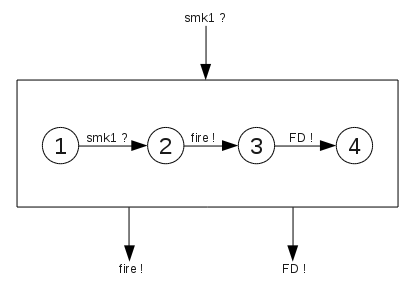
\includegraphics[scale=0.68]{fireDetector.png}
		\end{minipage}
		\hfill
		\begin{minipage}{0.3\linewidth}
		\centering 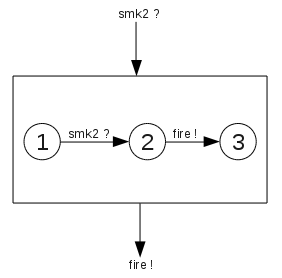
\includegraphics[scale=0.68]{controlUnit.png}
		\end{minipage}
		\caption{Detecteur de Fum�e}
	\end{center}
\end{figure}

\clearpage


\chapter{Construction d'automates d'interfaces}

Le but principal du projet est, partant d'un diagramme de d�finition de blocs, de r�cup�rer deux blocs interagissant ensembles et de pouvoir valider le fait qu'ils soient compatibles l'un avec l'autre.

Les automates d'interfaces des composants permettent de tester si deux composants sont compatibles. L'outil Ticc sera utilis� afin de tester la compatibilit� entre deux automates d'interfaces. 
Le diagramme de s�quences d'un bloc SysML est connu, il faut donc obtenir d'apr�s ce diagramme de s�quences, un fichier pouvant �tre lu par Ticc.
ATL entre en jeu � ce moment, il permet d'effectuer des transformations de mod�les : ici le passage d'un diagramme de s�quences � un fichier correspondant � la syntaxe de Ticc. 

\noindent En r�capitulant, pour tester la compatibilit� de deux blocs il faut :
\begin{itemize}
    \item g�n�rer un m�ta mod�le du diagramme de s�quences;
    \item g�n�rer un m�ta mod�le correspondant � la syntaxe de Ticc;
    \item �crire les r�gles ATL permettant le passage d'un diagramme de s�quences � un fichier Ticc;
    \item appliquer les r�gles ATL sur un fichier contenant les diagrammes de s�quences de deux blocs (appel�s par la suite composants), ce fichier doit �tre conforme au m�ta mod�le du diagramme de s�quences;
    \item parser le fichier obtenu apr�s application des r�gles pour obtenir un fichier compatible Ticc contenant les deux composants;
    \item g�n�rer un fichier d'ex�cution Ticc en OCaml;
    \item lancer le fichier d'ex�cution dans Ticc et conclure sur la compatibilit� des composants.

\end{itemize}

\section{Introduction {\`a} la transformation de mod{\`e}les}

Parmi les nombreux sujets de recherche existants, la conception et l'utilisation de mod{\`e}les font parti de ceux qui sont en pleine expansion. Le but de cette recherche {\'e}tant l'utilisation continue et syst{\'e}matique de ces mod{\`e}les tout au long d'un projet. L'un des aspects les plus importants {\'e}tant la g{\'e}n{\'e}ration et la transformation de mod{\`e}les {\`a} partir de r{\`e}gles. Il sera ainsi pr{\'e}sent{\'e} dans la suite de cette section, les diff{\'e}rentes approches de la transformation de mod{\`e}les, dont le but est d'introduire la transformation d'un diagramme de s{\'e}quence SysML vers un automate d'interfaces Ticc.

\subsection{Transformation endog{\`e}ne}

Une transformation endog{\`e}ne (ou raffinement) de mod{\`e}le consiste {\`a} modifier le contenu d'un mod{\`e}le sans en changer le but ou la s{\'e}mantique. Il s'agit de rajouter des d{\'e}tails {\`a} un mod{\`e}le ou bien de le restructurer pour en am{\'e}liorer la conception. Par principe, le raffinement implique que les deux mod{\`e}les, le mod{\`e}le source et le mod{\`e}le cible, soient du m{\^e}me type, c'est-{\`a}-dire conformes au m{\^e}me m{\'e}ta mod{\`e}le.

\noindent La figure~\ref{raffinement} ci-dessous repr{\'e}sente ce concept :

\begin{figure}[!ht]
	\centering
	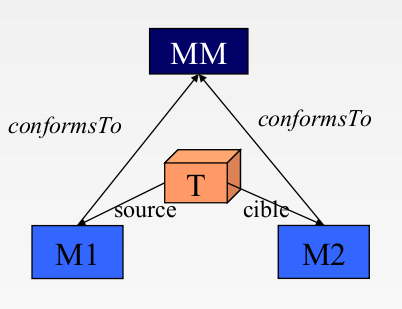
\includegraphics[scale=0.8]{endogene.png}
	\caption{Sch{\'e}ma d'une transformation endog{\`e}ne (ou par raffinement)}
	\label{raffinement}

\end{figure}

\subsection{Transformation exog{\`e}ne}

Il s'agit d'une transformation entre deux espaces technologiques diff{\'e}rents. Les mod{\`e}les source et cible sont conformes {\`a} des m{\'e}ta-mod{\`e}les diff{\'e}rents. Par exemple la conversion d'un fichier XML en un sch{\'e}ma BDD.

\noindent C'est cette configuration de transformation qui a {\'e}t{\'e} mise en {\oe}uvre dans le projet. La figure~\ref{projection} ci-dessous repr{\'e}sente ce concept : 

\begin{figure}[!ht]
	\centering
	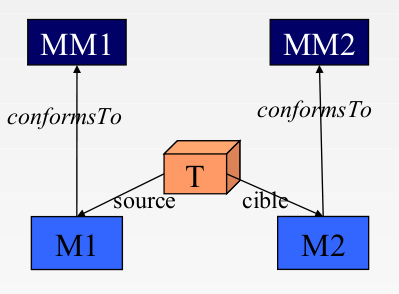
\includegraphics[scale=0.8]{exogene.png}
	\caption{Sch{\'e}ma d'une transformation exog{\`e}ne (ou par projection)}
	\label{projection}

\end{figure}

\subsection{Transformation g{\'e}n{\'e}rique}

Ce type de transformation se base sur les m{\'e}ta m{\'e}ta mod{\`e}les (mod{\`e}le MOF\protect\footnote{Meta-Object Facility}) et produit un mod{\`e}le cible g{\'e}n{\'e}rique, qui peut {\^e}tre r{\'e}utilisable. Elle peut {\^e}tre exog{\`e}ne ou endog{\`e}ne.

\subsection{Query}

La transformation de mod{\`e}le query est un type de transformation qui permet la transformation d'un m{\'e}ta mod{\`e}le en texte (documentation ou code source).

\noindent Par exemple :
\begin{itemize}
	\item transformer un mod{\`e}le UML vers du code Java;
	\item contr{\^o}ler la coh{\'e}rence d'un mod{\`e}le UML en �crivant une transformation qui affiche un diagnostic.
	
\end{itemize}

\section{R�alisation}

\subsection{ATL : un choix technique}

L'utilisation d'ATL, pour la r�cup�ration et le traitement d'un fichier Ticc contenant deux composants, requiert :
\begin{itemize}
    \item deux m�ta mod�les en entr�e : un de base (celui du diagramme de s�quences) et un d'arriv� (celui du langage Ticc);
    \item un fichier conforme au m�ta mod�le de base;
    \item les r�gles ATL permettant de passer du m�ta mod�le de base au m�ta mod�le voulu.

\end{itemize}

\subsection{Les m�ta mod�les}

\subsubsection{M�ta mod�le du diagramme de s�quences}
\label{subsubMMDiagSeq}

Le m�ta mod�le de s�quence existant n'a pas �t� pris dans son ensemble, seules les parties importantes ont �t� extraites.
Par principe, les messages �chang�s se font entre un composant et son environnement.

\noindent Les ensembles de messages pris en compte sont :
\begin{itemize}
    \item \textbf{alt} : messages multiples alternatifs (si alors sinon);
    \item \textbf{loop} : messages s'ex�cutant plusieurs fois (boucle);
    \item \textbf{seq} : messages n'ayant pas d'ordre particulier.

\end{itemize}

Ces ensembles peuvent contenir eux-m�mes d'autres ensembles contenant des messages. Un message est compos� d'un �metteur et d'un r�cepteur. Il poss�de aussi une m�thode associ�e qui poss�de un nom.

Une s�quence type pour le diagramme de s�quences, dont il est question d'utiliser dans le cadre du projet, sera compos�e de diff�rents composants \textit{NamedElement}, de messages \textit{Message} et �ventuellement d'ensembles de messages \textit{TypeMessage}.
La figure~\ref{figureMMDiagSeq} repr�sente le m�ta mod�le r�fl�chit dans le cadre du projet.

\begin{figure}[!ht]
	\centering
	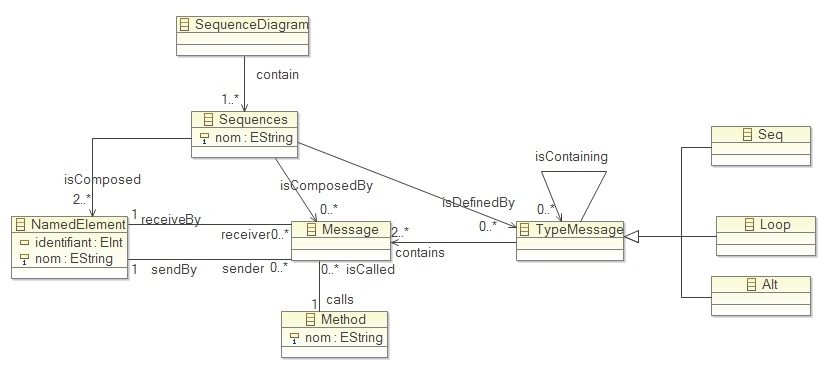
\includegraphics[scale=0.62]{MMDiagSeq.jpg}
	\caption{M�ta mod�le du diagramme de s�quences utile pour le projet}
	\label{figureMMDiagSeq}

\end{figure}

\subsubsection{M�ta mod�le du langage de Ticc}

Concernant Ticc, le m�ta mod�le a �t� cr�� en se basant sur la syntaxe du logiciel et apr�s analyse des fichiers exemples. En effet, Ticc permet de traiter des automates d�t sociaux, pouvant communiquer entre eux. Or cette notion n'est pas utile dans le cadre du projet, elle a donc, de ce fait, �t� �cart�e du m�ta mod�le.

Le code ci-dessous repr�sente comme vu dans la partie~\ref{utilisationTicc} un module.
\lstinputlisting{./doc/moduleExemple.si}

Un module porte un nom et est donc compos� d'un tableau repr�sentant les diff�rents �tats de l'automate. Il peut aussi avoir un �tat initial.
Il contient ensuite les diff�rentes transitions possibles de l'automate :
\begin{itemize}
	\item \textbf{Input} une transition d'entr�e de l'automate qui peut �tre d�compos�e en deux types :
	\begin{itemize}
		\item[$\bullet$] \textbf{GlobalInput} principalement utilis�e pour les automates sociaux, elle peut repr�senter aussi des entr�es ne faisant pas changer l'�tat de l'automate;
		\item[$\bullet$] \textbf{LocalInput} cette transition repr�sente une entr�e dans l'automate entrainant ou non un changement d'�tat interne.
	
	\end{itemize}
	\item \textbf{Output} une transition de sortie de l'automate;
	\item \textbf{Local} une transition interne de l'automate.
				
\end{itemize}

Dans le cas d'un changement d'�tat, l'�tat suivant est not� d'un \' (voir l'exemple ci-dessus avec \textbf{s'}).

\clearpage

\noindent La figure~\ref{figureMMTicc} repr�sente le m�ta mod�le r�fl�chit dans le cadre du projet.

\begin{figure}[!ht]
	\centering
	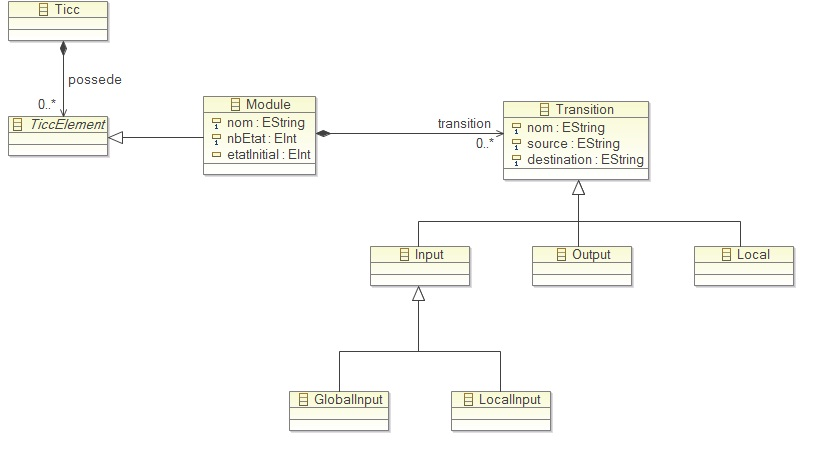
\includegraphics[scale=0.62]{MMTicc.jpg}
	\caption{M�ta mod�le de la syntaxe de Ticc utile pour le projet}
	\label{figureMMTicc}

\end{figure}

%TODO a completer avec reference fichier Ticc

\subsection{Les r�gles ATL}

Apr�s g�n�ration des deux m�ta mod�les intervient l'�criture des r�gles ATL permettant le passage d'un diagramme de s�quences � un automate d'interface.

Un algorithme permettant le passage d'un diagramme de s�quences en un automate d'interface �tait fourni en d�but de projet. Cependant l'application d'un algorithme it�ratif r�cursif en r�gles ATL n'est pas possible du fait de la conception d'ATL utilisant EMF\protect\footnote{Eclipse Modeling Framework : framework de mod�lisation d'eclipse} qui utilise des mod�les de donn�es structur�es.

Pour l'ex�cution d'ATL, ce qu'il faut savoir c'est qu'il prend en entr�e un fichier de type \textit{XMI}\protect\footnote{XML Metadata Interchange : format standard de repr�sentation de mod�les UML bas� sur XML} et g�n�re en sortie un fichier du m�me type.

Comme annonc� en d�but de~\ref{subsubMMDiagSeq}, les �changes d'un composant se font entre lui et un composant abstrait appel� \textit{Environnement}. Il repr�sente tous les autres composants �mettant ou r�ceptionnant des messages du composant �tudi� dans la s�quence. La figure~\ref{diagSeqExemple} permet d'illustrer un �change de ce type.

\begin{figure}[!ht]
    \centering
    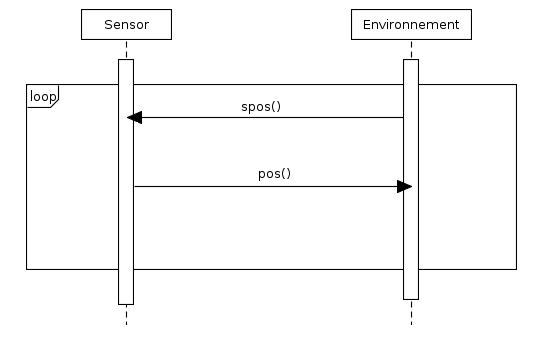
\includegraphics[scale=0.5]{diagSeqExemple.png}
    \caption{Exemple de diagramme de s�quences}
    \label{diagSeqExemple}

\end{figure}

En reprenant les deux m�ta mod�les vus pr�c�demment (figures~\ref{figureMMDiagSeq} et~\ref{figureMMTicc}), on peut constater des similitudes qui permettent de faire les transformations. La figure~\ref{figureSimilitude} permet d'avoir, via des m�ta mod�les simplifi�s, une vue des �l�ments qui subiront une transformation avec une r�gle ATL.

\begin{figure}[!ht]
    \centering
    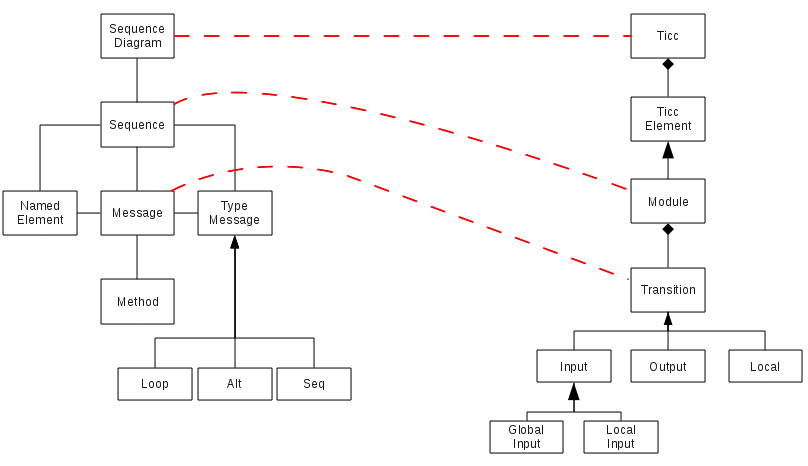
\includegraphics[scale=0.5]{figureSimilitudeSeqTicc.png}
    \caption{Similitude du m�ta mod�le du diagramme de s�quences avec celui de Ticc}
    \label{figureSimilitude}

\end{figure}

\noindent Les r�gles sont les suivantes : 
\begin{itemize}
	\item Le diagramme de s�quences devient un mod�le Ticc, toutes les s�quences qu'il contient deviennent des �l�ments de type module que poss�de le mod�le Ticc;
	\item Une s�quence du diagramme de s�quence devient un module :
    \begin{itemize}
        \item[$\bullet$] le nom du module est le m�me que celui de la s�quence;
        \item[$\bullet$] le nombre d'�tats poss�d� correspond au nombre de \textit{NamedElement};
        \item[$\bullet$] l'�tat initial correspond � l'�metteur du premier message de la s�quence;
        \item[$\bullet$] les transitions du mod�le Ticc sont en correspondance avec les �l�ments de type \textit{Message} du mod�le du diagramme de s�quences.

    \end{itemize}

    \item Un message devient une transition de type \textit{LocalInput} ou \textit{Output} en fonction de l'�metteur ou du r�cepteur du message :
    \begin{itemize}
        \item[$\bullet$] il devient une transition \textit{LocalInput} si l'�metteur du message est le \textit{NamedElement} nomm� \textit{Environnement};
        \item[$\bullet$] il devient une transition \textit{Output} si le r�cepteur du message est le \textit{NamedElement} nomm� \textit{Environnement};
        \item[$\bullet$] le nom de la transition est celui de la m�thode qu'appelle le message;
        \item[$\bullet$] la source et la destination d'une transition sont respectivement l'�metteur et le receveur d'un message.

    \end{itemize}

\end{itemize}

Pour la validit� de ces r�gles, il convient bien s�r que seuls les messages �mis par le composant voulu et les messages qu'il re�oit sont int�ressant. Les autres sont ignor�s.

% ANNEXE !!!!
Le fichier d'entr�e exemple, le fichier des r�gles ATL et le fichier de sortie sont disponibles en annexe (\ref{fichierExempleEntree}, \ref{regleATL} et \ref{fichierExempleSortie}).

\subsection{Parseur XML vers Ticc}

Afin de pouvoir utiliser Ticc pour v�rifier la compatibilit� des composants, il est n�cessaire de convertir le fichier XMI obtenu en sortie en un fichier .si compatible avec Ticc. Pour ce faire, un parseur XML a �t� impl�ment�. 
Il permet de r�cup�rer un fichier XMI en entr�e, et s'il est syntaxiquement correcte, un fichier .si associ� est g�n�r� ainsi qu'un fichier d'ex�cution .in. Ces fichiers peuvent eux aussi �tre trouv�s en annexe (\ref{fichierParseSI} et \ref{fichierParseIN}).

\label{compatibiliteAutomate}

\subsection{Processus de transformation}

Comme d�j� �tabli tout au long du rapport, le sch�ma~\ref{ProcessusTransformation} ci-dessous permet de visualiser les diff�rentes �tapes de transformations de mod�les, ainsi que l'impl�mentation r�alis�e dans le projet. 

\begin{figure}[!ht]
	\centering
	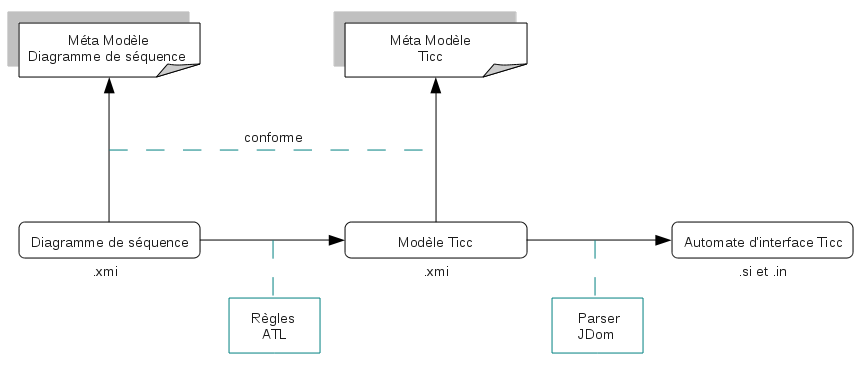
\includegraphics[scale=0.7]{ProcessusTransformation2.png}
	\caption{Processus de transformation d'un diagramme SysML en automate d'interface Ticc}
	\label{ProcessusTransformation}

\end{figure}

Le diagramme de s�quence traduit en fichier XMI suit les r�gles ATL pour �tre transform� en mod�le Ticc �galement sous format XMI. A l'aide d'un parseur JDom, le mod�le Ticc est transform� sous la syntaxe Ticc en un automate d'interface. Le fichier executable .in produit peut ensuite �tre interpr�t� par Ticc pour la v�rification de la compatibilit�.

\clearpage


\chapter{V�rification de compatibilit� entre composants}

\section{Automate d'interfaces}

La notion d'automate d'interfaces a �t� introduite par Alfaro et Henzinger~\cite{automataInterface} dans le but de mod�liser les interfaces des composants et de d�crire l'enchainement des appels de services. Ces automates sont issus des automates de type entr�e/sortie~\cite{automateIO} o� il n'est pas n�cessaire d'avoir des actions d'entr�e activables dans tous les �tats.

Chaque composant est d�crit par un seul automate d'interfaces. 
L'ensemble des actions est d�compos� en trois ensembles : 
\begin{itemize}
	\item les actions d'entr�e repr�sentant les services offerts (identifiable par le caract�re \enquote{?}) correspondant aux r�ceptions de messages;
	\item les actions de sortie repr�sentant les services requis (identifiable par le caract�re \enquote{!}) correspondant aux envois de messages;
	\item et les actions internes repr�sentant des op�rations locales (identifiable par le caract�re \enquote{;}).

\end{itemize}

\noindent La figure~\ref{exempleAutomateInterface} donne un exemple de repr�sentation d'automates d'interfaces.

\begin{figure}[!ht]
	\centering
	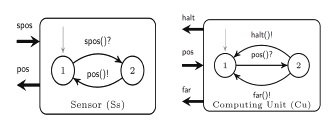
\includegraphics[scale=1]{exempleAutomateInterface.jpg}
	\caption{Repr�sentation d'automates d'interfaces}
	\label{exempleAutomateInterface}

\end{figure}

\noindent Un automate d'interfaces $ A = \{S_A, I_A, \Sigma_A^I, \Sigma_A^O, \Sigma_A^H, \mathcal{T}_A\} $ est d�fini par :
\begin{itemize}
    \item un ensemble fini d'�tats $S_A$;
    \item un sous-ensemble fini d'�tats initiaux $I_A$ tel que $I_A \subseteq S_A$;
    \item un ensemble d'actions d'entr�e $\Sigma_A^I$;
    \item un ensemble d'actions de sortie $\Sigma_A^0$;
    \item un ensemble d'actions internes $\Sigma_A^H$;
    \item un ensemble $\mathcal{T}_A \subseteq S_A \times \Sigma_A \times S_A$ de transitions entre �tats.

\end{itemize}

\section{Compatibilit� entre composants}

V�rifier la compatibilit� entre deux composants revient � v�rifier la compatibilit� entre leur deux automates d'interfaces respectif. Cependant, la v�rification de cette compatibilit� n�cessite diff�rentes �tapes interm�diaires.

\subsection{Composabilit� de composants}

Il faut commencer par v�rifier que les deux automates sont composables, c'est � dire que leurs ensembles d'actions d'entr�e, de sortie et internes sont disjoints.

Deux automates d'interfaces P et Q sont composables si :
\begin{center}
	\begin{tabular}{l c}
		$\Sigma_P^H  \cap \Sigma_Q = \emptyset$ &
		$\Sigma_Q^H  \cap \Sigma_P = \emptyset$ \\
		$\Sigma_P^I  \cap \Sigma_Q^I = \emptyset$ &
		$\Sigma_P^O  \cap \Sigma_Q^O = \emptyset$ \\
			
	\end{tabular}				

\end{center}

\subsection{Produit synchronis� de composants}

L'�tape suivante consiste � faire le produit synchronis� des deux automates et v�rifier qu'il ne poss�de pas d'�tats d�t ill�gaux : ce sont des �tats � partir desquels une action de sortie partag�e d'un automate ne peut pas �tre synchronis�e avec la m�me action activ�e en entr�e dans l'autre composant.

Le produit synchronis� de deux automate d'interfaces P et Q  not� $A_P \otimes A_Q$ est d�fini par :
\begin{itemize}
	\item[$\bullet$] $S_{P \otimes Q} = S_P \times S_Q et I_{P \otimes Q} = I_P \times I_Q$;
	\item[$\bullet$] $\Sigma_{P \otimes Q}^I = (\Sigma_P^I \cup \Sigma_Q^I) \setminus Shared(P,Q)$;
	\item[$\bullet$] $\Sigma_{P \otimes Q}^O = (\Sigma_P^O \cup \Sigma_Q^O) \setminus Shared(P,Q)$;
	\item[$\bullet$] $\Sigma_{P \otimes Q}^H = (\Sigma_P^H \cup \Sigma_Q^H) \setminus Shared(P,Q)$;
	\item[$\bullet$] $((s_1,s_2),a,(s_1^{'},s_2^{'})) \in \mathcal{T}_{P \otimes Q}$ si :
	\begin{itemize}
		\item $a \notin Shared(P,Q) \wedge (s_1,a,s_1^{'}) \in \mathcal{T}_P \wedge s_2 = s_2^{'}$;
		\item $a \notin Shared(P,Q) \wedge (s_2,a,s_2^{'}) \in \mathcal{T}_Q \wedge s_1 = s_1^{'}$;
		\item $a \in Shared(P,Q) \wedge (s_1,a,s_1^{'}) \in \mathcal{T}_P \wedge (s_2,a,s_2^{'}) \in \mathcal{T}_Q$.
	
	\end{itemize}
		
\end{itemize}
Avec $Shared(P,Q) = \Sigma_P \cap \Sigma_Q$.

\subsection{Notion d'�tats ill�gaux}

Les �tats ill�gaux entre deux automates d'interfaces P et Q sont d�finis par :
\begin{center} 
	{\footnotesize	$Illegal(P,Q) = \left\{(v,u) \in S_P \times S_Q \mid 
		\exists a \in Shared(P,Q).
		\left(\begin{array}{l l l}
			a \in \Sigma_P^O(v) & \wedge & a \notin \Sigma_Q^I(u) \\
			& \vee &\\
			a \in \Sigma_Q^O(u) & \wedge & a \notin \Sigma_P^I(v)
		\end{array}\right)\right\}$}.\\

		Avec $Shared(P,Q) = \Sigma_P \cap \Sigma_Q$.

\end{center}

\subsection{Compatibilit� entre deux composants}

Deux automates d'interfaces sont incompatibles s'il existe un �tat ill�gal atteignable depuis les �tats initiaux dans le produit synchronis� de deux composants.


\subsection{Compatibilit� des automates d'interfaces avec Ticc}

Pour v�rifier la compatibilit� des automates d'interfaces via l'outil Ticc~\cite{ticcDocumentation, siteTicc}, il faut lancer le fichier .in. Ce fichier r�alise la composition des interfaces deux � deux et affiche le r�sultat.

\clearpage


\chapter{Probl�mes rencontr�s}

Durant le projet, divers probl�mes sont apparus. Plus ou moins complexes � r�soudre, ils n'ont n�anmoins pas emp�ch� la r�alisation de celui-ci.

Le premier probl�me fut de tenter de transposer l'algorithme fourni dans les r�gles ATL. Il est apparu que ce n'�tait pas possible du fait de la conception du langage ATL. Les r�gles propres aux m�ta mod�les ont donc �t� impl�ment�es.
Ensuite est apparu un probl�me technique concernant le site de Ticc. %mettre la r�f�rence � la bibliographie
Le site n'�tait plus accessible d'acc�s, ce qui incluait donc plus de documentations le concernant. Par chance, le logiciel en lui-m�me avait d�j� �t� r�cup�r� pour pouvoir travailler dessus.

Suite � la transformation de mod�les, la transcription du fichier g�n�r� en syntaxe Ticc et l'ex�cution du code OCamL, s'est pos� le probl�me de savoir comment traiter le r�sultat obtenu. En effet, Ticc permet l'affichage de la compatibilit� de deux automates, cependant, cet affichage est une tentative d'assemblage des deux automates et la sortie g�n�r�e est cons�quente.

\clearpage


\chapter{Conclusion et perspectives}

Le langage de mod�lisation SysML connait un succ�s grandissant dans le milieu industriel et acad�mique du fait des am�liorations qu'il apporte par rapport � UML. Il permet de donner � un projet, une vue d'ensemble des interactions entre blocs. Cependant, il ne permet pas de v�rifier si ces interactions sont correctes.

D'un autre c�t�, dans le domaine des composants, il est possible de sp�cifier des automates d'interface correspondants. Ces automates contiennent les diff�rentes actions, internes, d'entr�e et de sortie du composant. Les recherches sur le sujet de L. Alfaro et T. Henzinger ont permis de d�finir ces automates et ouvert la voie � la v�rification de la compatibilit� entre composants. Cette v�rification est bas�e sur la composition des interfaces et sur la synchronisation des actions des composants. Si deux automates d'interface sont compatibles, leurs composants associ�s le seront aussi.
L.Alfaro et T. Henzinger ont ainsi d�velopp� un logiciel nomm� Ticc permettant d'interagir avec des automates d'interface et de tester la compatibilit� entre deux composants.

Ainsi pour tester la compatibilit� de deux blocs SysML, il suffit de transformer le diagramme de s�quences associ� � chaque bloc en un automate d'interface et de v�rifier la compatibilit� des automates.

La partie �tude du projet a donc �t� consacr�e � la transformation de mod�le dans une premi�re partie. Cette partie permettant � partir d'un m�ta mod�le du diagramme de s�quences, d'un fichier conforme � ce m�ta mod�le et de r�gles ATL de g�n�rer un fichier conforme � un m�ta mod�le correspondant � la syntaxe de Ticc. 
La seconde partie ouvre la voie � la v�rification de compatibilit� d'automates, le fichier g�n�r� � partir d'ATL est, apr�s traitement, ex�cutable par Ticc. 

Par la suite, il est possible de cr�er un plugin eclipse permettant d'effectuer la d�marche de fa�on automatique afin de donner un r�sultat pour la compatibilit� de deux blocs SysML. Ce plugin pourra �tre coupl� avec un algorithme de parcours de blocs et de ce fait donnera pour un diagramme de blocs complet une r�ponse concernant la compatibilit�. 


\clearpage


%%%%%----------------------------------------
%%%%% Pour la bibliographie
%%%%%----------------------------------------
%%%%% Citer tous les ouvrages/rfrences
\nocite{*}
%%%%% Trier par ordre d'apparition
\bibliographystyle{unsrt}
%%%%% Pour le style de la biblio
%\bibliographystyle{plain}
%%%%% Ecrire la biblio ici
\bibliography{Bibliographie}
\addcontentsline{toc}{chapter}{Bibliographie}
\clearpage

\printindex

\appendix

\listoffigures
\addcontentsline{toc}{chapter}{Table des figures}
\clearpage

\begin{appendices}

\lstset{
    basicstyle=\small,
	numbers=left,
	numberstyle=\footnotesize,
	stepnumber=2,
	numbersep=5pt,
	frame=shadowbox,
	backgroundcolor=\color{grisclair},
	rulesepcolor=\color{gris}
}

\chapter{Exemple de fichier d'entr�e conforme au m�ta mod�le du diagramme de s�quences}
\label{fichierExempleEntree}

\lstinputlisting{./doc/DiagSeqEntree.xmi}


\chapter{Exemple de fichier de sortie conforme � la syntaxe de Ticc}
\label{fichierExempleSortie}

\lstinputlisting{./doc/Resultat.xmi}

\chapter{R�gles ATL de transformation}
\label{regleATL}

\lstinputlisting{./doc/SequenceToTicc.atl}


\chapter{Exemple de fichier Ticc apr�s parsage (modules)}
\label{fichierParseSI}

\lstinputlisting{./doc/ticcFile.si}


\chapter{Exemple de fichier Ticc apr�s parsage (ex�cutable OCamL)}
\label{fichierParseIN}

\lstinputlisting{./doc/ticcFile.in}


\end{appendices}

\clearpage


\end{document}
